%-----------------------------------------------------------------------------%
\chapter{\babTiga}
\label{bab:3}

Bab ini secara umum memaparkan tentang metodologi penelitian yang ditempuh dalam mengembangkan sistem PeerToCP yang mencakup pendekatan, rincian tahapan, serta aspek-aspek yang akan diujikan pada sistem. Pendekatan dan tahapan penelitian penting untuk memberikan penjelasan terhadap langkah-langkah saintifik yang ditempuh dalam penelitian ini.

\section{Pendekatan dan Tahapan Penelitian}
\label{sec:pendekatan}
Penelitian ini dilaksanakan dengan pendekatan \textit{experimental research}. Data kuantitatif dan kualitatif diukur untuk setiap variasi dari aplikasi PeerToCP yang memiliki implementasi \textit{business logic} di atas UI (\textit{user interface}) atau antarmuka pengguna yang sama. Variabel bebas dari penelitian ini difokuskan pada basis arsitektur dari jaringan PeerToCP serta metode resolusi dan sinkronisasi data yang digunakan. Variabel terikat yang diukur dari penelitian ini disusun berdasarkan aspek-aspek sistem. Data kuantitatif didapat dari hasil \textit{benchmarking} dan dianalisis . Data kualitatif didapatkan melalui paparan deskriptif secara objektif terhadap sistem. Bagan berikut memberikan gambaran besar tahapan penelitian yang dilaksanakan.

\begin{figure}
    \centering
    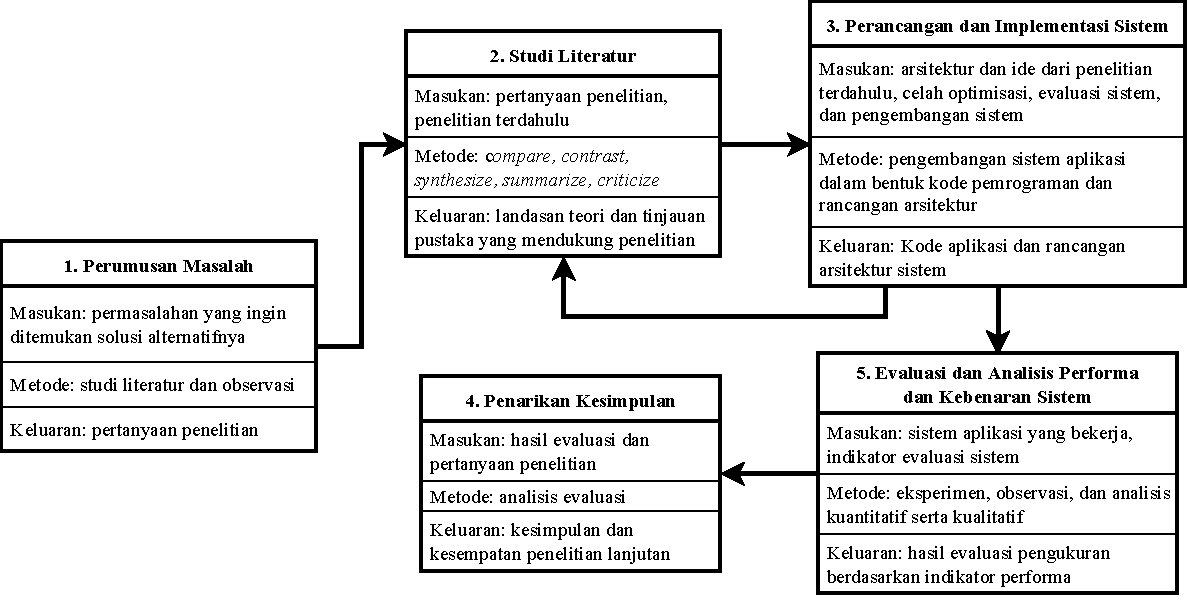
\includegraphics[scale=0.7]{assets/skripsi/Metode_Penelitian}
    \caption{Bagan Alur Penelitian}
    \label{bagan}
\end{figure}

Perumusan masalah dalam penelitian ini dilatarbelakangi oleh potensi penggunaan teknologi web berupa WebRTC dan beberapa variasi algoritma sinkronisasi data dalam suatu jaringan terdistribusi yang memiliki keuntungan dan kerugiannya masing-masing. Ide ini dikembangkan pula melalui kebutuhan sistem yang mempermudah melakukan kegiatan pemrograman kompetitif, yaitu suatu IDE (\textit{Integrated Development Environment}) sederhana yang memungkinkan adanya pengembangan kode secara kolaboratif dalam waktu nyata dan penjalanan program yang dapat dilakukan pada suatu klien di dalam jaringan yang dapat diakses oleh setiap klien lain di dalam jaringan pula. Dari rumusan masalah tersebut, didapatkan pertanyaan-pertanyaan yang mendasari penelitian ini.

Melalui masukan pertanyaan, dilakukan studi literatur terhadap teknologi-teknologi dan penelitian terdahulu. Tahap ini menghasilkan landasan teori dan tinjauan pustaka sebagai dasar pengetahuan. Studi literatur dilakukan dengan membandingkan penelitian terkait yang serupa, dari segi performa, kerumitan implementasi, cara kerja, dan bukti kebenaran teknologi atau algoritma tertentu. Studi literatur ini berguna untuk mengetahui seberapa jauh kemajuan teknologi yang diteliti pada topik ini. Selanjutnya, penelitian dilanjutkan dengan perancangan dan implementasi sistem aplikasi PeerToCP. Terdapat tiga variasi dari sistem aplikasi PeerToCP yang diujikan, yaitu variasi dengan metode OT (\textit{operational transformation}) berbasis \textit{client-server}, CRDT (\textit{conflict-free replicated data types}) berbasis \textit{client-server}, dan CRDT berbasis \textit{peer-to-peer}. Sistem yang telah dikembangkan kemudian dievaluasi secara objektif berdasarkan aspek-aspek tertentu yang merepresentasikan performa dan skalabilitas aplikasi. Poin-poin aspek yang disampaikan pada subbab~\ref{sec:evaluasi} selanjutnya disampakan untuk memberikan konteks perbandingan yang jelas antara suatu implementasi dengan yang lainnya.

\section{Metode dan Skenario Evaluasi}
\label{sec:evaluasi}

Dari observasi terhadap beberapa aplikasi \textit{real-time collaborative} lain, evaluasi pada penelitian ini mengikutsertakan beberapa aspek esensial untuk setiap variasi dari aplikasi PeerToCP, antara lain ialah sebagai berikut.

\begin{enumerate}
    \item \textit{Correctness}, mengindikasikan kebenaran untuk setiap variasi implementasi PeerToCP. Aspek ini dipilih untuk menentukan bahwa setiap replika data yang dijaga kesamaannya berakhir konvergen dan identik.
    \item \textit{Lightweight}, aplikasi berjalan dengan sumber daya atau \textit{resource} minimal dan tidak mengganggu jalannya aplikasi lain pada suatu sistem operasi. Suatu aplikasi hendaknya tidak menggunakan \textit{resource} yang berlebihan dalam mencapai tujuannya, hal ini dapat berdampak langsung terhadap minat penggunaan aplikasi ke depannya.
    \item \textit{Responsiveness}, sinkronisasi replika data pada setiap klien dilakukan dalam latensi yang rendah dan layak guna. Setiap klien yang menggunakan suatu aplikasi \textit{real-time collaborative} seharusnya mendapatkan jeda minimal untuk memberikan pengalaman pengguna atau \textit{user experience} waktu nyata.
    \item \textit{Local-First}, operasi diterapkan pada replika lokal secara langsung setelah diberikan pengguna tanpa perlu berhubungan dengan klien atau server lain di dalam jaringan.
    \item \textit{Scalability}, aspek ini berhubungan langsung dengan setiap aspek lain, karena penggunaan arsitektur \textit{peer-to-peer} pada awalnya memiliki motivasi untuk meningkatkan ketersediaan layanan dengan mengurangi beban pada server. Performa dari aplikasi berpengaruh terhadap banyaknya klien atau pengguna dalam suatu jaringan, sehingga aspek ini penting untuk diperhatikan dalam sistem terdistribusi aplikasi~\citep{leibnitz2007peer}.
\end{enumerate}

Data kuantitatif dan kualitatif yang diperoleh pada proses \textit{benchmarking} ini dianalisis. Setelahnya, hasil analisis disimpulkan dengan memberikan kesempatan optimisasi dan pengembangan untuk penelitian-penelitian selanjutnya.
